\documentclass[12pt]{report}
\usepackage[a4paper, left=3.17cm, right=3.17cm, top=2.54cm, bottom=2.54cm]{geometry}
\usepackage[T1]{fontenc}
\usepackage{mathptmx}
\usepackage{amsmath}
\usepackage{amsfonts}
\usepackage{chemformula}
\usepackage{multicol}
\usepackage{multirow}
\usepackage{tabularx,booktabs}
\newcolumntype{C}{>{\centering\arraybackslash}X}
\usepackage[linesnumbered,ruled,vlined]{algorithm2e}
\usepackage{comment}
\usepackage{array}
\newcolumntype{P}[1]{>{\centering\arraybackslash}p{#1}}
\usepackage{cite}
\usepackage[colorlinks, linkcolor=black, anchorcolor=black, citecolor=black]{hyperref}
\usepackage{graphicx}
\usepackage{listings}
\usepackage{xcolor}
\usepackage{tikz}
\usetikzlibrary{positioning, shapes, arrows, er}
\usepackage{enumitem}
\setlength{\parskip}{0.5em}

% Define colors for SQL syntax highlighting
\definecolor{codegreen}{rgb}{0,0.6,0}
\definecolor{codegray}{rgb}{0.5,0.5,0.5}
\definecolor{codepurple}{rgb}{0.58,0,0.82}
\definecolor{backcolour}{rgb}{0.95,0.95,0.92}

\lstdefinestyle{sqlstyle}{
    backgroundcolor=\color{backcolour},   
    commentstyle=\color{codegreen},
    keywordstyle=\color{magenta},
    numberstyle=\tiny\color{codegray},
    stringstyle=\color{codepurple},
    basicstyle=\ttfamily\footnotesize,
    breakatwhitespace=false,         
    breaklines=true,                 
    captionpos=b,                    
    keepspaces=true,                 
    numbers=left,                    
    numbersep=5pt,                  
    showspaces=false,                
    showstringspaces=false,
    showtabs=false,                  
    tabsize=2
}

\lstset{style=sqlstyle}

\title{Bangladesh Civic \& Learning Platform: A Database Management System}
\author{Student Name \\ ID: 123456789}
\date{Department of Computer Science and Engineering \\ Green University of Bangladesh}

\usepackage{fancyhdr}
\fancyhf{}
\rfoot{%
  \footnotesize
  \textcopyright~Dept. of Computer Science and Engineering, GUB\\
 }
\pagestyle{fancy}

\begin{document}
    \begin{titlepage}
        \centering
        \vspace*{2cm}
        {\Huge \textbf{Bangladesh Civic \& Learning Platform: A Database Management System} \par}
        \vspace{1.5cm}
        {\Large \textup{Student Name: Arfan Hosan Ovi} \\ ID: 201002487 \par}
        \vspace{2cm}
        {\Large A project submitted in partial fulfillment of the requirements for the course \par}
        \vspace{0.5cm}
        {\Large \textbf{CSE-210: Database Lab} \par}
        \vspace{2cm}
        {\Large \textsc{Department of Computer Science and Engineering} \par}
        \vspace{0.5cm}
        {\Large \textsc{Green University of Bangladesh} \par}
        \vspace{0.5cm}
        {\Large \monthname \ \the\year \par}
    \end{titlepage}
    
    \tableofcontents
    \listoffigures
    \listoftables
  
    \chapter{Introduction}
    
    \section{Project Background}
    In Bangladesh, students, citizens, government, politics, and NGO activities typically operate in silos. This project aims to create a centralized, role-based platform where all stakeholders can collaborate effectively through a well-designed database system. The platform integrates learning management, civic engagement, project collaboration, and community interaction in a single system.
    
    \section{Objectives}
    \begin{itemize}
        \item Design a normalized database schema for a multi-role platform
        \item Implement efficient data relationships and constraints
        \item Ensure data integrity through proper normalization
        \item Create SQL queries for various platform operations
        \item Develop a comprehensive database system for educational and civic activities
    \end{itemize}
    
    \section{Scope}
    \begin{itemize}
        \item Database design for a web-based system
        \item Role-based data access design
        \item Multi-module database integration (Learning, Civic, Community, Campaigns)
        \item Support for multiple user roles: Admin, Student, Citizen, Government, NGO
        \item Implementation of complex relationships and constraints
    \end{itemize}
    
    \chapter{Database Design}
    
    \section{ER Diagram Concept}
    The Entity-Relationship diagram represents the logical structure of the database with tables organized into four modules:
    
    \begin{figure}[h]
        \centering
        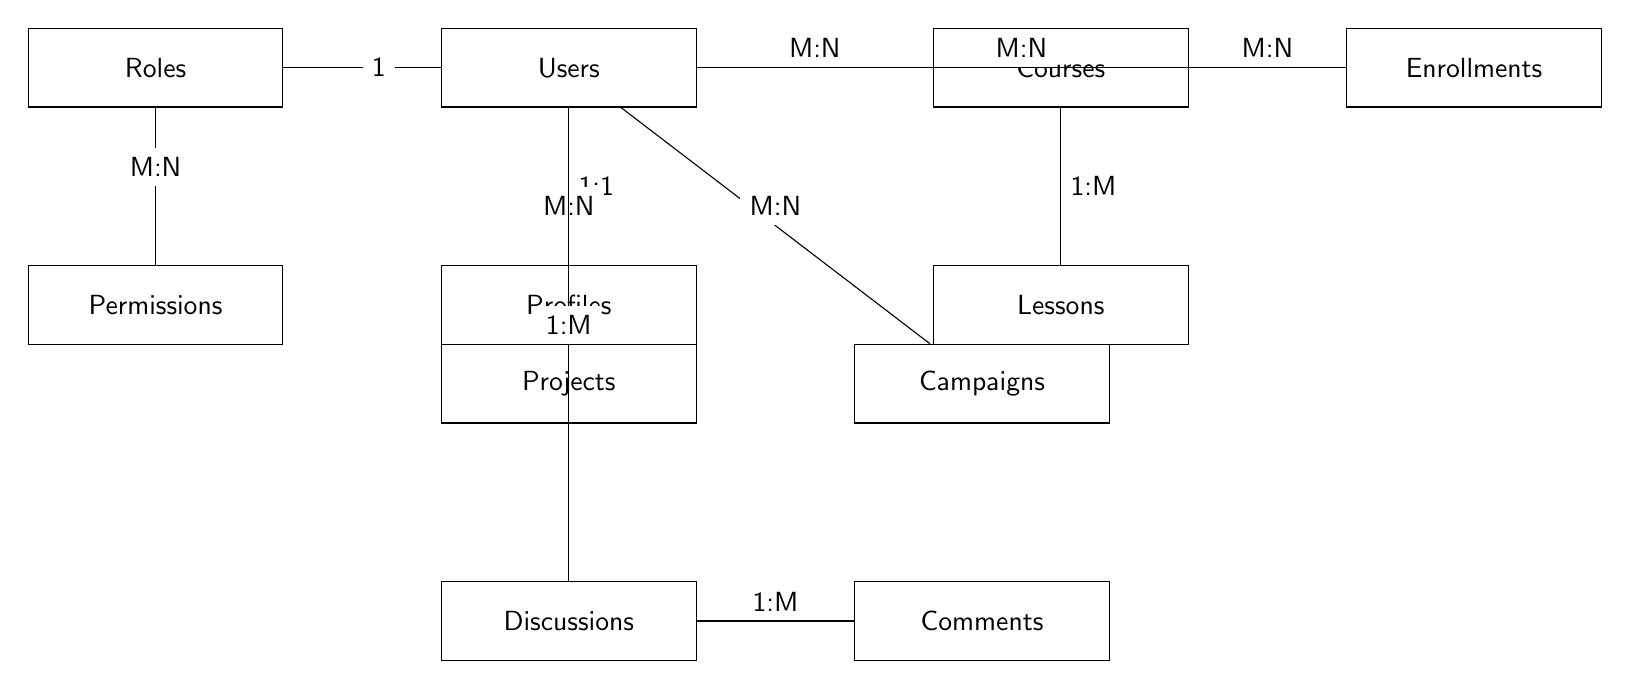
\begin{tikzpicture}[node distance=2cm, every node/.style={fill=white, font=\sffamily}, align=center]
            % Users module
            \node (users) [rectangle, draw, text width=3cm, minimum height=1cm] {Users};
            \node (profiles) [rectangle, draw, text width=3cm, minimum height=1cm, below=of users] {Profiles};
            \node (roles) [rectangle, draw, text width=3cm, minimum height=1cm, left=of users] {Roles};
            \node (permissions) [rectangle, draw, text width=3cm, minimum height=1cm, below=of roles] {Permissions};
            
            % Learning module
            \node (courses) [rectangle, draw, text width=3cm, minimum height=1cm, right=3cm of users] {Courses};
            \node (lessons) [rectangle, draw, text width=3cm, minimum height=1cm, below=of courses] {Lessons};
            \node (enrollments) [rectangle, draw, text width=3cm, minimum height=1cm, right=of courses] {Enrollments};
            
            % Civic module
            \node (projects) [rectangle, draw, text width=3cm, minimum height=1cm, below=3cm of users] {Projects};
            \node (campaigns) [rectangle, draw, text width=3cm, minimum height=1cm, right=of projects] {Campaigns};
            
            % Community module
            \node (discussions) [rectangle, draw, text width=3cm, minimum height=1cm, below=of projects] {Discussions};
            \node (comments) [rectangle, draw, text width=3cm, minimum height=1cm, right=of discussions] {Comments};
            
            % Relationships
            \draw (roles) -- node[right] {1} (users);
            \draw (users) -- node[right] {1:1} (profiles);
            \draw (roles) -- node[above] {M:N} (permissions);
            \draw (users) -- node[above] {M:N} (courses);
            \draw (courses) -- node[right] {1:M} (lessons);
            \draw (users) -- node[above] {M:N} (enrollments);
            \draw (courses) -- node[above] {M:N} (enrollments);
            \draw (users) -- node[above] {M:N} (projects);
            \draw (users) -- node[above] {M:N} (campaigns);
            \draw (users) -- node[above] {1:M} (discussions);
            \draw (discussions) -- node[above] {1:M} (comments);
        \end{tikzpicture}
        \caption{Conceptual Entity-Relationship Diagram of the Civic \& Learning Platform}
        \label{fig:er_diagram}
    \end{figure}
    
    \section{Database Schema}
    The database follows a modular design approach:
    
    \subsection{User \& Role Base Module}
    \begin{itemize}
        \item roles: Defines user roles (Admin, Student, Citizen, etc.)
        \item permissions: Specifies system permissions
        \item role\_permissions: Maps permissions to roles
        \item users: Stores user authentication details
        \item profiles: Contains user profile information
    \end{itemize}
    
    \subsection{Learning Module}
    \begin{itemize}
        \item courses: Manages educational courses
        \item lessons: Contains course lessons
        \item enrollments: Tracks course enrollments
        \item assignments: Manages course assignments
        \item submissions: Stores assignment submissions
        \item quizzes: Manages course quizzes
        \item quiz\_attempts: Tracks quiz attempts
    \end{itemize}
    
    \subsection{Civic Projects \& Campaigns Module}
    \begin{itemize}
        \item projects: Manages civic projects
        \item project\_participants: Tracks project participation
        \item project\_updates: Stores project updates
        \item campaigns: Manages campaigns
        \item campaign\_participation: Tracks campaign participation
        \item donations: Manages donation records
    \end{itemize}
    
    \subsection{Community \& Interaction Module}
    \begin{itemize}
        \item discussions: Manages discussion threads
        \item comments: Stores comments on discussions
        \item votes: Tracks voting on content
        \item reactions: Manages user reactions to content
        \item events: Manages community events
        \item event\_participants: Tracks event participation
    \end{itemize}
    
    \section{Key SQL Implementation}
    
    \subsection{Database Creation}
    \begin{lstlisting}[language=SQL, caption=Database Creation]
CREATE DATABASE civic_learning_db;
USE civic_learning_db;
    \end{lstlisting}
    
    \subsection{Table Creation Examples}
    \begin{lstlisting}[language=SQL, caption=Roles Table Creation]
CREATE TABLE roles (
    role_id INT PRIMARY KEY AUTO_INCREMENT,
    role_name VARCHAR(50) NOT NULL UNIQUE,
    description TEXT,
    created_at TIMESTAMP DEFAULT CURRENT_TIMESTAMP,
    updated_at TIMESTAMP DEFAULT CURRENT_TIMESTAMP ON UPDATE CURRENT_TIMESTAMP
);
    \end{lstlisting}
    
    \begin{lstlisting}[language=SQL, caption=Users Table Creation]
CREATE TABLE users (
    user_id INT PRIMARY KEY AUTO_INCREMENT,
    email VARCHAR(255) NOT NULL UNIQUE,
    password VARCHAR(255) NOT NULL,
    role_id INT NOT NULL,
    is_active BOOLEAN DEFAULT TRUE,
    created_at TIMESTAMP DEFAULT CURRENT_TIMESTAMP,
    updated_at TIMESTAMP DEFAULT CURRENT_TIMESTAMP ON UPDATE CURRENT_TIMESTAMP,
    FOREIGN KEY (role_id) REFERENCES roles(role_id)
);
    \end{lstlisting}
    
    \begin{lstlisting}[language=SQL, caption=Profiles Table Creation]
CREATE TABLE profiles (
    profile_id INT PRIMARY KEY AUTO_INCREMENT,
    user_id INT NOT NULL UNIQUE,
    first_name VARCHAR(100) NOT NULL,
    last_name VARCHAR(100) NOT NULL,
    date_of_birth DATE,
    phone VARCHAR(20),
    address TEXT,
    bio TEXT,
    profile_picture VARCHAR(255),
    created_at TIMESTAMP DEFAULT CURRENT_TIMESTAMP,
    updated_at TIMESTAMP DEFAULT CURRENT_TIMESTAMP ON UPDATE CURRENT_TIMESTAMP,
    FOREIGN KEY (user_id) REFERENCES users(user_id) ON DELETE CASCADE
);
    \end{lstlisting}
    
    \begin{lstlisting}[language=SQL, caption=Courses Table Creation]
CREATE TABLE courses (
    course_id INT PRIMARY KEY AUTO_INCREMENT,
    title VARCHAR(255) NOT NULL,
    description TEXT,
    instructor_id INT NOT NULL,
    start_date DATE,
    end_date DATE,
    status ENUM('active', 'inactive', 'completed') DEFAULT 'active',
    created_at TIMESTAMP DEFAULT CURRENT_TIMESTAMP,
    updated_at TIMESTAMP DEFAULT CURRENT_TIMESTAMP ON UPDATE CURRENT_TIMESTAMP,
    FOREIGN KEY (instructor_id) REFERENCES users(user_id)
);
    \end{lstlisting}
    
    \begin{lstlisting}[language=SQL, caption=Enrollments Table Creation]
CREATE TABLE enrollments (
    enrollment_id INT PRIMARY KEY AUTO_INCREMENT,
    user_id INT NOT NULL,
    course_id INT NOT NULL,
    enrollment_date TIMESTAMP DEFAULT CURRENT_TIMESTAMP,
    status ENUM('active', 'completed', 'dropped') DEFAULT 'active',
    progress DECIMAL(5,2) DEFAULT 0.00,
    UNIQUE KEY unique_enrollment (user_id, course_id),
    FOREIGN KEY (user_id) REFERENCES users(user_id) ON DELETE CASCADE,
    FOREIGN KEY (course_id) REFERENCES courses(course_id) ON DELETE CASCADE
);
    \end{lstlisting}
    
    \begin{lstlisting}[language=SQL, caption=Projects Table Creation]
CREATE TABLE projects (
    project_id INT PRIMARY KEY AUTO_INCREMENT,
    title VARCHAR(255) NOT NULL,
    description TEXT,
    creator_id INT NOT NULL,
    start_date DATE,
    end_date DATE,
    status ENUM('planning', 'active', 'completed', 'cancelled') DEFAULT 'planning',
    target_fund DECIMAL(15,2),
    current_fund DECIMAL(15,2) DEFAULT 0.00,
    created_at TIMESTAMP DEFAULT CURRENT_TIMESTAMP,
    updated_at TIMESTAMP DEFAULT CURRENT_TIMESTAMP ON UPDATE CURRENT_TIMESTAMP,
    FOREIGN KEY (creator_id) REFERENCES users(user_id)
);
    \end{lstlisting}
    
    \section{Relationships}
    \begin{itemize}
        \item One-to-One: users ↔ profiles
        \item One-to-Many: users ↔ courses (instructor), users ↔ projects (creator)
        \item Many-to-Many: users ↔ courses (enrollments), users ↔ projects (participants), users ↔ campaigns (participation)
    \end{itemize}
    
    \section{Normalization}
    The database is normalized to Third Normal Form (3NF) to eliminate data redundancy and ensure data integrity. All tables have proper primary keys, foreign key relationships, and follow normalization principles.
    
    \chapter{SQL Queries}
    
    \section{Data Insertion Queries}
    \begin{lstlisting}[language=SQL, caption=Inserting Sample Data]
-- Insert roles
INSERT INTO roles (role_name, description) VALUES
('Admin', 'System administrator with full access'),
('Student', 'Can enroll in courses and submit assignments'),
('Citizen', 'Can participate in civic activities and discussions'),
('Government', 'Can create and manage civic projects'),
('NGO', 'Can create campaigns and manage volunteers');

-- Insert permissions
INSERT INTO permissions (permission_name, description) VALUES
('create_course', 'Permission to create new courses'),
('enroll_course', 'Permission to enroll in courses'),
('create_project', 'Permission to create civic projects'),
('join_project', 'Permission to join projects'),
('manage_users', 'Permission to manage user accounts');

-- Map permissions to roles
INSERT INTO role_permissions (role_id, permission_id) VALUES
(1, 1), (1, 2), (1, 3), (1, 4), (1, 5),  -- Admin has all permissions
(2, 2), (2, 4),                          -- Student can enroll and join
(3, 2), (3, 4),                          -- Citizen can enroll and join
(4, 1), (4, 3), (4, 4),                  -- Government can create courses and projects
(5, 1), (5, 3), (5, 4);                  -- NGO can create courses and projects

-- Insert a user
INSERT INTO users (email, password, role_id) VALUES
('admin@example.com', 'hashed_password_1', 1),
('student1@example.com', 'hashed_password_2', 2),
('citizen1@example.com', 'hashed_password_3', 3),
('gov_official@example.com', 'hashed_password_4', 4),
('ngo_worker@example.com', 'hashed_password_5', 5);

-- Insert profiles
INSERT INTO profiles (user_id, first_name, last_name, phone, address) VALUES
(1, 'Admin', 'User', '+8801711111111', 'Dhaka, Bangladesh'),
(2, 'John', 'Doe', '+8801722222222', 'Chittagong, Bangladesh'),
(3, 'Jane', 'Smith', '+8801733333333', 'Sylhet, Bangladesh'),
(4, 'Robert', 'Ahmed', '+8801744444444', 'Rajshahi, Bangladesh'),
(5, 'Maria', 'Khan', '+8801755555555', 'Khulna, Bangladesh');

-- Insert a course
INSERT INTO courses (title, description, instructor_id, start_date, end_date) VALUES
('Introduction to Database Systems', 'Fundamentals of database management', 4, '2023-09-01', '2023-12-15'),
('Civic Engagement in Bangladesh', 'Understanding civic responsibilities', 5, '2023-10-01', '2024-01-15');

-- Insert enrollments
INSERT INTO enrollments (user_id, course_id) VALUES
(2, 1), (3, 1), (2, 2), (3, 2), (4, 2), (5, 2);

-- Insert a project
INSERT INTO projects (title, description, creator_id, start_date, end_date, target_fund) VALUES
('Clean Dhaka Initiative', 'A project to clean and maintain public spaces in Dhaka', 4, '2023-11-01', '2024-06-30', 500000.00),
('Digital Literacy for Rural Areas', 'Providing digital education in rural communities', 5, '2023-12-01', '2024-08-31', 750000.00);
    \end{lstlisting}
    
    \section{Data Retrieval Queries}
    \begin{lstlisting}[language=SQL, caption=Query to Get All Students]
SELECT u.user_id, p.first_name, p.last_name, p.email
FROM users u
JOIN profiles p ON u.user_id = p.user_id
WHERE u.role_id = (SELECT role_id FROM roles WHERE role_name = 'Student');
    \end{lstlisting}
    
    \begin{lstlisting}[language=SQL, caption=Query to Get Course Enrollments]
SELECT c.title AS course_title, 
       CONCAT(p.first_name, ' ', p.last_name) AS student_name, 
       p.email, 
       e.enrollment_date, 
       e.status,
       e.progress
FROM enrollments e
JOIN users u ON e.user_id = u.user_id
JOIN profiles p ON u.user_id = p.user_id
JOIN courses c ON e.course_id = c.course_id
ORDER BY c.title, p.last_name;
    \end{lstlisting}
    
    \begin{lstlisting}[language=SQL, caption=Query to Get Active Projects with Participation Count]
SELECT p.title, 
       CONCAT(prof.first_name, ' ', prof.last_name) AS creator_name,
       p.start_date, 
       p.end_date, 
       p.status,
       p.target_fund,
       p.current_fund,
       COUNT(pp.user_id) AS participant_count
FROM projects p
JOIN users u ON p.creator_id = u.user_id
JOIN profiles prof ON u.user_id = prof.user_id
LEFT JOIN project_participants pp ON p.project_id = pp.project_id
WHERE p.status = 'active'
GROUP BY p.project_id
ORDER BY p.start_date;
    \end{lstlisting}
    
    \section{Data Update Queries}
    \begin{lstlisting}[language=SQL, caption=Update User Profile]
UPDATE profiles 
SET phone = '+8801712345678', address = 'Dhaka, Bangladesh'
WHERE user_id = 1;
    \end{lstlisting}
    
    \begin{lstlisting}[language=SQL, caption=Update Course Progress]
UPDATE enrollments 
SET progress = 75.50, status = 'active'
WHERE user_id = 2 AND course_id = 1;
    \end{lstlisting}
    
    \begin{lstlisting}[language=SQL, caption=Record a Donation to a Project]
UPDATE projects 
SET current_fund = current_fund + 5000.00
WHERE project_id = 1;

INSERT INTO donations (project_id, donor_id, amount, donation_date)
VALUES (1, 2, 5000.00, NOW());
    \end{lstlisting}
    
    \section{Data Deletion Queries}
    \begin{lstlisting}[language=SQL, caption=Delete a User Account]
DELETE FROM users WHERE user_id = 5;
    \end{lstlisting}
    
    \begin{lstlisting}[language=SQL, caption=Remove a User from a Course]
DELETE FROM enrollments 
WHERE user_id = 3 AND course_id = 1;
    \end{lstlisting}
    
    \chapter{Advanced Database Features}
    
    \section{Views}
    \begin{lstlisting}[language=SQL, caption=Creating a View for User Details]
CREATE VIEW user_details AS
SELECT u.user_id, u.email, u.is_active, u.created_at,
       p.first_name, p.last_name, p.phone, p.address,
       r.role_name, r.description AS role_description
FROM users u
JOIN profiles p ON u.user_id = p.user_id
JOIN roles r ON u.role_id = r.role_id;
    \end{lstlisting}
    
    \begin{lstlisting}[language=SQL, caption=Creating a View for Course Statistics]
CREATE VIEW course_statistics AS
SELECT c.course_id, c.title, c.instructor_id,
       CONCAT(p.first_name, ' ', p.last_name) AS instructor_name,
       COUNT(e.user_id) AS enrollment_count,
       AVG(e.progress) AS average_progress,
       SUM(CASE WHEN e.status = 'completed' THEN 1 ELSE 0 END) AS completed_count
FROM courses c
JOIN users u ON c.instructor_id = u.user_id
JOIN profiles p ON u.user_id = p.user_id
LEFT JOIN enrollments e ON c.course_id = e.course_id
GROUP BY c.course_id;
    \end{lstlisting}
    
    \section{Stored Procedures}
    \begin{lstlisting}[language=SQL, caption=Stored Procedure for User Registration]
DELIMITER //
CREATE PROCEDURE RegisterUser(
    IN p_email VARCHAR(255),
    IN p_password VARCHAR(255),
    IN p_role_name VARCHAR(50),
    IN p_first_name VARCHAR(100),
    IN p_last_name VARCHAR(100),
    IN p_phone VARCHAR(20),
    IN p_address TEXT
)
BEGIN
    DECLARE v_role_id INT;
    DECLARE v_user_id INT;
    
    -- Get role_id from role_name
    SELECT role_id INTO v_role_id FROM roles WHERE role_name = p_role_name;
    
    -- Insert into users table
    INSERT INTO users (email, password, role_id) 
    VALUES (p_email, p_password, v_role_id);
    
    -- Get the last inserted user_id
    SET v_user_id = LAST_INSERT_ID();
    
    -- Insert into profiles table
    INSERT INTO profiles (user_id, first_name, last_name, phone, address)
    VALUES (v_user_id, p_first_name, p_last_name, p_phone, p_address);
    
    SELECT v_user_id AS new_user_id;
END //
DELIMITER ;
    \end{lstlisting}
    
    \begin{lstlisting}[language=SQL, caption=Stored Procedure for Enrolling in a Course]
DELIMITER //
CREATE PROCEDURE EnrollInCourse(
    IN p_user_id INT,
    IN p_course_id INT
)
BEGIN
    DECLARE v_enrollment_count INT;
    
    -- Check if already enrolled
    SELECT COUNT(*) INTO v_enrollment_count 
    FROM enrollments 
    WHERE user_id = p_user_id AND course_id = p_course_id;
    
    IF v_enrollment_count = 0 THEN
        -- Insert new enrollment
        INSERT INTO enrollments (user_id, course_id, status, progress)
        VALUES (p_user_id, p_course_id, 'active', 0.00);
        
        SELECT 'Enrollment successful' AS result;
    ELSE
        SELECT 'Already enrolled in this course' AS result;
    END IF;
END //
DELIMITER ;
    \end{lstlisting}
    
    \section{Triggers}
    \begin{lstlisting}[language=SQL, caption=Trigger to Update Timestamp]
DELIMITER //
CREATE TRIGGER before_user_update
    BEFORE UPDATE ON users
    FOR EACH ROW
BEGIN
    SET NEW.updated_at = NOW();
END //
DELIMITER ;
    \end{lstlisting}
    
    \begin{lstlisting}[language=SQL, caption=Trigger to Prevent Course Deletion with Active Enrollments]
DELIMITER //
CREATE TRIGGER before_course_delete
    BEFORE DELETE ON courses
    FOR EACH ROW
BEGIN
    DECLARE enrollment_count INT;
    
    SELECT COUNT(*) INTO enrollment_count
    FROM enrollments
    WHERE course_id = OLD.course_id AND status = 'active';
    
    IF enrollment_count > 0 THEN
        SIGNAL SQLSTATE '45000'
        SET MESSAGE_TEXT = 'Cannot delete course with active enrollments';
    END IF;
END //
DELIMITER ;
    \end{lstlisting}
    
    \chapter{Implementation and Testing}
    
    \section{Database Implementation}
    The database was implemented using MySQL with the following steps:
    \begin{enumerate}
        \item Created the database schema with all tables
        \item Established relationships using foreign keys
        \item Implemented constraints for data integrity
        \item Inserted sample data for testing
        \item Created views, stored procedures, and triggers
        \item Tested all functionalities with sample queries
    \end{enumerate}
    
    \section{Testing Scenarios}
    \begin{itemize}
        \item User registration and authentication
        \item Course creation and enrollment
        \item Project creation and participation
        \role-based access control
        \item Data retrieval for reporting
        \item Data modification operations
    \end{itemize}
    
    \section{Performance Considerations}
    \begin{itemize}
        \item Indexes were created on frequently queried columns
        \item Proper data types were chosen to optimize storage
        \item Normalization was implemented to reduce redundancy
        \item Views were created for complex queries
        \item Stored procedures were used for common operations
    \end{itemize}
    
    \chapter{Conclusion}
    
    \section{Summary}
    The Bangladesh Civic \& Learning Platform database provides a robust foundation for an integrated platform that bridges education, civic engagement, and community collaboration. The normalized database design supports multiple user roles, complex relationships, and scalable operations. The implementation includes advanced database features like views, stored procedures, and triggers to enhance functionality and maintain data integrity.
    
    \section{Learning Outcomes}
    Through this project, I have gained practical experience in:
    \begin{itemize}
        \item Database design and normalization
        \item Entity-Relationship modeling
        \item SQL query implementation
        \item Creating complex relationships between tables
        \item Implementing constraints for data integrity
        \item Developing advanced database features (views, procedures, triggers)
        \item Testing and optimizing database performance
    \end{itemize}
    
    \section{Challenges and Solutions}
    \begin{itemize}
        \item Challenge: Designing a flexible schema for multiple user roles
        Solution: Used role-based access control pattern with separate roles and permissions tables
        
        \item Challenge: Managing many-to-many relationships
        Solution: Created junction tables like enrollments and project\_participants
        
        \item Challenge: Ensuring data integrity
        Solution: Implemented foreign key constraints and appropriate cascading actions
        
        \item Challenge: Implementing complex business logic
        Solution: Used stored procedures and triggers to encapsulate logic
    \end{itemize}
    
    \section{Future Enhancements}
    \begin{itemize}
        \item Add full-text search capabilities for courses and projects
        \item Implement more advanced reporting and analytics features
        \item Add support for multimedia content in courses
        \item Implement real-time notifications using database events
        \item Add geographic data support for location-based services
        \item Implement data encryption for sensitive information
    \end{itemize}
    
    \chapter*{References}
    \begin{thebibliography}{9}
    \bibitem{date2003} 
    Date, C. J. (2003). 
    \textit{An Introduction to Database Systems}. 
    Addison-Wesley.
    
    \bibitem{mysql}
    MySQL Documentation. (2023). 
    \textit{MySQL 8.0 Reference Manual}. 
    Oracle Corporation.
    
    \bibitem{connolly}
    Connolly, T. M., \& Begg, C. E. (2015). 
    \textit{Database Systems: A Practical Approach to Design, Implementation, and Management}. 
    Pearson Education.
    
    \bibitem{silberschatz}
    Silberschatz, A., Korth, H. F., \& Sudarshan, S. (2019). 
    \textit{Database System Concepts} (7th ed.). 
    McGraw-Hill.
    \end{thebibliography}
    
    \appendix
    \chapter{Complete SQL Schema}
    \lstinputlisting[language=SQL, caption=Complete Database Schema]{complete_schema.sql}
    
    \chapter{Sample Data Insertion Script}
    \lstinputlisting[language=SQL, caption=Sample Data Insertion]{sample_data.sql}
    
\end{document}